\documentclass[10pt]{article}

\usepackage[utf8]{inputenc}
\usepackage{color,verbatim,Sweave,url,xargs,amsmath,hyperref,booktabs,longtable}
\usepackage[left=2cm,right=2cm,top=2cm,bottom=2cm]{geometry}
\usepackage{fancyhdr}
\pagestyle{fancy}
\fancyhf{}
\lhead{\textsc{BHCC Mat-181}}
\rhead{\textsc{Homework due Sept 5th}}

\usepackage{caption}
\captionsetup[figure]{labelformat=empty}

\usepackage{float}
\floatplacement{figure}{H}


%% new environments
\newenvironment{question}{\item \textbf{Problem}\newline}{}
\newenvironment{solution}{\textbf{Solution}\newline}{\newpage}
\newenvironment{answerlist}{\renewcommand{\labelenumi}{(\alph{enumi})}\begin{enumerate}}{\end{enumerate}}


%% compatibility with pandoc
\providecommand{\tightlist}{\setlength{\itemsep}{0pt}\setlength{\parskip}{0pt}}

%% fonts: Helvetica
\renewcommand{\sfdefault}{phv}
\IfFileExists{sfmath.sty}{
  \RequirePackage[helvet]{sfmath}
  \renewcommand{\rmdefault}{phv}
}{}

\newcommand{\extext}[1]{\textbf{\large #1}}
\newcommandx{\exmchoice}[9][2=-,3=-,4=-,5=-,6=-,7=-,8=-,9=-]{%
                \mbox{(a) \,\, \framebox[8mm]{\rule[-1mm]{0mm}{5mm} \hspace*{-1.6mm} \extext{#1}} \hspace*{2mm}}%
  \if #2- \else \mbox{(b) \,\, \framebox[8mm]{\rule[-1mm]{0mm}{5mm} \hspace*{-1.6mm} \extext{#2}} \hspace*{2mm}} \fi%
  \if #3- \else \mbox{(c) \,\, \framebox[8mm]{\rule[-1mm]{0mm}{5mm} \hspace*{-1.6mm} \extext{#3}} \hspace*{2mm}} \fi%
  \if #4- \else \mbox{(d) \,\, \framebox[8mm]{\rule[-1mm]{0mm}{5mm} \hspace*{-1.6mm} \extext{#4}} \hspace*{2mm}} \fi%
  \if #5- \else \mbox{(e) \,\, \framebox[8mm]{\rule[-1mm]{0mm}{5mm} \hspace*{-1.6mm} \extext{#5}} \hspace*{2mm}} \fi%
  \if #6- \else \mbox{(f) \,\, \framebox[8mm]{\rule[-1mm]{0mm}{5mm} \hspace*{-1.6mm} \extext{#6}} \hspace*{2mm}} \fi%
  \if #7- \else \mbox{(g) \,\, \framebox[8mm]{\rule[-1mm]{0mm}{5mm} \hspace*{-1.6mm} \extext{#7}} \hspace*{2mm}} \fi%
  \if #8- \else \mbox{(h) \,\, \framebox[8mm]{\rule[-1mm]{0mm}{5mm} \hspace*{-1.6mm} \extext{#8}} \hspace*{2mm}} \fi%
  \if #9- \else \mbox{(i) \,\, \framebox[8mm]{\rule[-1mm]{0mm}{5mm} \hspace*{-1.6mm} \extext{#9}} \hspace*{2mm}} \fi%
}
\newcommandx{\exclozechoice}[9][2=-,3=-,4=-,5=-,6=-,7=-,8=-,9=-]{\setcounter{enumiii}{1}%
                \mbox{\roman{enumiii}. \, \framebox[8mm]{\rule[-1mm]{0mm}{5mm} \hspace*{-1.6mm} \extext{#1}} \hspace*{2mm}\stepcounter{enumiii}}%
  \if #2- \else \mbox{\roman{enumiii}. \, \framebox[8mm]{\rule[-1mm]{0mm}{5mm} \hspace*{-1.6mm} \extext{#2}} \hspace*{2mm}\stepcounter{enumiii}} \fi%
  \if #3- \else \mbox{\roman{enumiii}. \, \framebox[8mm]{\rule[-1mm]{0mm}{5mm} \hspace*{-1.6mm} \extext{#3}} \hspace*{2mm}\stepcounter{enumiii}} \fi%
  \if #4- \else \mbox{\roman{enumiii}. \, \framebox[8mm]{\rule[-1mm]{0mm}{5mm} \hspace*{-1.6mm} \extext{#4}} \hspace*{2mm}\stepcounter{enumiii}} \fi%
  \if #5- \else \mbox{\roman{enumiii}. \, \framebox[8mm]{\rule[-1mm]{0mm}{5mm} \hspace*{-1.6mm} \extext{#5}} \hspace*{2mm}\stepcounter{enumiii}} \fi%
  \if #6- \else \mbox{\roman{enumiii}. \, \framebox[8mm]{\rule[-1mm]{0mm}{5mm} \hspace*{-1.6mm} \extext{#6}} \hspace*{2mm}\stepcounter{enumiii}} \fi%
  \if #7- \else \mbox{\roman{enumiii}. \, \framebox[8mm]{\rule[-1mm]{0mm}{5mm} \hspace*{-1.6mm} \extext{#7}} \hspace*{2mm}\stepcounter{enumiii}} \fi%
  \if #8- \else \mbox{\roman{enumiii}. \, \framebox[8mm]{\rule[-1mm]{0mm}{5mm} \hspace*{-1.6mm} \extext{#8}} \hspace*{2mm}\stepcounter{enumiii}} \fi%
  \if #9- \else \mbox{\roman{enumiii}. \, \framebox[8mm]{\rule[-1mm]{0mm}{5mm} \hspace*{-1.6mm} \extext{#9}} \hspace*{2mm}} \fi%
}
\newcommand{\exnum}[9]{%
  \mbox{\framebox[8mm]{\rule[-1mm]{0mm}{5mm} \hspace*{-1.6mm} \extext{#1}}}%
  \mbox{\framebox[8mm]{\rule[-1mm]{0mm}{5mm} \hspace*{-1.6mm} \extext{#2}}}%
  \mbox{\framebox[8mm]{\rule[-1mm]{0mm}{5mm} \hspace*{-1.6mm} \extext{#3}}}%
  \mbox{\framebox[8mm]{\rule[-1mm]{0mm}{5mm} \hspace*{-1.6mm} \extext{#4}}}%
  \mbox{\framebox[8mm]{\rule[-1mm]{0mm}{5mm} \hspace*{-1.6mm} \extext{#5}}}%
  \mbox{\framebox[8mm]{\rule[-1mm]{0mm}{5mm} \hspace*{-1.6mm} \extext{#6}}}%
  \mbox{ \makebox[3mm]{\rule[-1mm]{0mm}{5mm} \hspace*{-2mm} .}}%
  \mbox{\framebox[8mm]{\rule[-1mm]{0mm}{5mm} \hspace*{-1.6mm} \extext{#7}}}%
  \mbox{\framebox[8mm]{\rule[-1mm]{0mm}{5mm} \hspace*{-1.6mm} \extext{#8}}}%
  \mbox{\framebox[8mm]{\rule[-1mm]{0mm}{5mm} \hspace*{-1.6mm} \extext{#9}}}%
}
\newcommand{\exstring}[1]{%
  \mbox{\framebox[0.9\textwidth][l]{\rule[-1mm]{0mm}{5mm} \hspace*{-1.6mm} \extext{#1}} \hspace*{2mm}}%
}

%% new commands
\makeatletter
\newcommand{\ID}[1]{\def\@ID{#1}}
\newcommand{\Date}[1]{\def\@Date{#1}}
\ID{00001}
\Date{YYYY-MM-DD}

\Date{2019-09-04}
\ID{008}

\newcommand{\myID}{\@ID}
\newcommand{\myDate}{\@Date}
\makeatother

%% headings
\lhead{\textsc{BHCC Mat-181}}
\rhead{\textsc{Homework due Sept 5th, ID = \myID}}


\begin{document}

\begin{enumerate}


\begin{question}
Please make a frequency table and a dot plot from the following
(unsorted) data.

\begin{longtable}[]{@{}rrrrr@{}}
\toprule
\endhead
17 & 17 & 16 & 15 & 13\tabularnewline
16 & 13 & 14 & 14 & 17\tabularnewline
18 & 15 & 18 & 17 & 11\tabularnewline
15 & 16 & 18 & 15 & 12\tabularnewline
\bottomrule
\end{longtable}
\end{question}

\begin{solution}
Make a frequency table.

\begin{longtable}[]{@{}rr@{}}
\toprule
value & frequency\tabularnewline
\midrule
\endhead
11 & 1\tabularnewline
12 & 1\tabularnewline
13 & 2\tabularnewline
14 & 2\tabularnewline
15 & 4\tabularnewline
16 & 3\tabularnewline
17 & 4\tabularnewline
18 & 3\tabularnewline
\bottomrule
\end{longtable}

Make the dot plot.

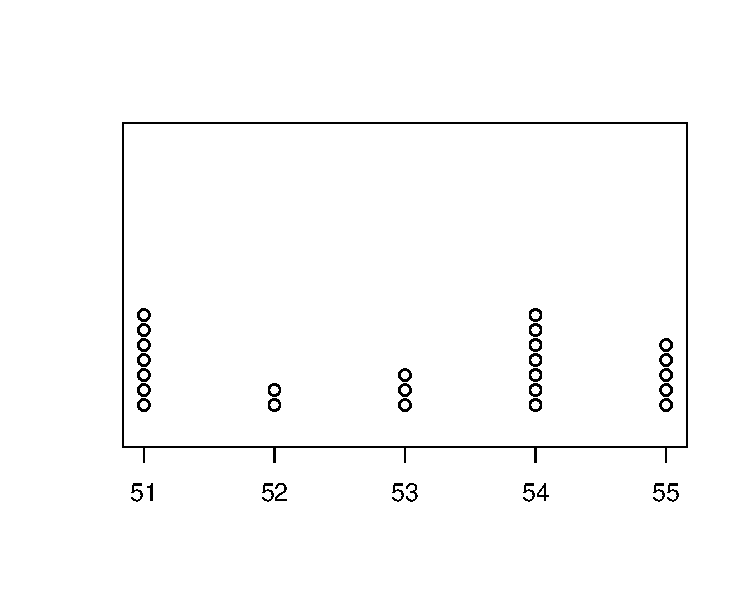
\includegraphics{hist-1.pdf}\\
\end{solution}



\begin{question}
Please make a frequency histogram from the following (unsorted)
continuous data by rounding to the nearest integer.

\begin{longtable}[]{@{}rrrrrr@{}}
\toprule
32.8201 & 27.7238 & 26.8074 & 29.1022 & 26.8669 & 31.1417\tabularnewline
27.2485 & 29.5684 & 32.2030 & 28.2653 & 27.0917 & 31.5793\tabularnewline
29.1215 & 27.6318 & 27.4419 & 29.8927 & 32.5300 & 26.7177\tabularnewline
30.3773 & 31.1362 & 30.5521 & 30.5156 & 31.8444 & 31.9692\tabularnewline
30.1981 & 31.9197 & 31.0182 & 31.5077 & 30.5075 & 28.5467\tabularnewline
\bottomrule
\end{longtable}
\end{question}

\begin{solution}
Make a frequency table.

\begin{longtable}[]{@{}rr@{}}
\toprule
value & frequency\tabularnewline
\midrule
\endhead
27 & 6\tabularnewline
28 & 3\tabularnewline
29 & 3\tabularnewline
30 & 4\tabularnewline
31 & 6\tabularnewline
32 & 6\tabularnewline
33 & 2\tabularnewline
\bottomrule
\end{longtable}

Make the histogram.

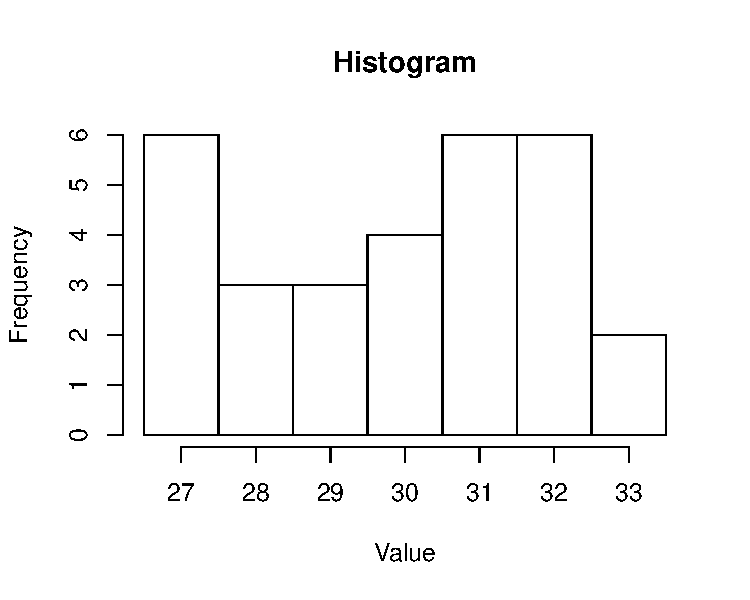
\includegraphics{barchart-1.pdf}\\
\end{solution}



\end{enumerate}



\end{document}
